\section{User Interface Representation}
UI design of our project is really simple which can be easily understood by a layman.
\begin{figure}[h!]
\centering 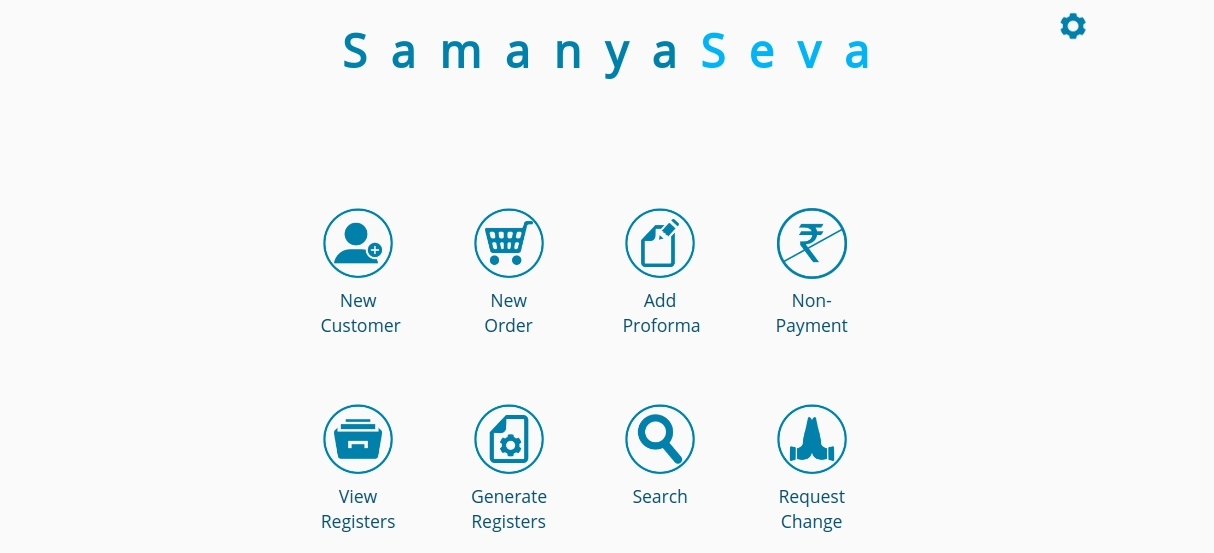
\includegraphics[scale=0.4]{input/images/samanya1.png}
\caption{ UI}
\label{fig:UI1}
\end{figure}

\begin{figure}[h!]
\centering \includegraphics[scale=0.4]{input/images/ui.png}
\caption{ User Interface}
\label{fig:UI1}
\end{figure}

\section{ Brief Description of Various Modules of the system}
\subsection{UserAccounts}
In this module, admin can check user data which were added while adding a new customer/user. Addition of users contains many fields like First and last name, Telephone, GST Number, Username and Password.

\begin{figure}[h!]
\centering 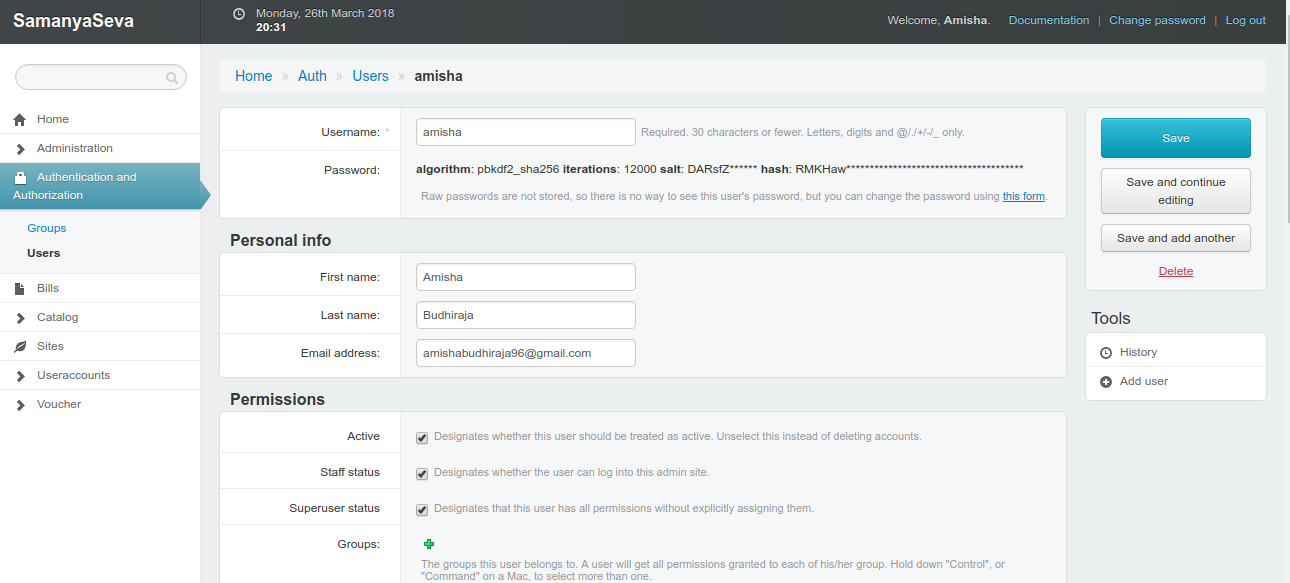
\includegraphics[scale=0.4]{input/images/after_customer_added.png}
\caption{ UserAccounts}
\label{fig:UI1}
\end{figure}

\subsection{Bills}
User can add a particular payment mode, as per user convinience.

\begin{figure}[h!]
\centering 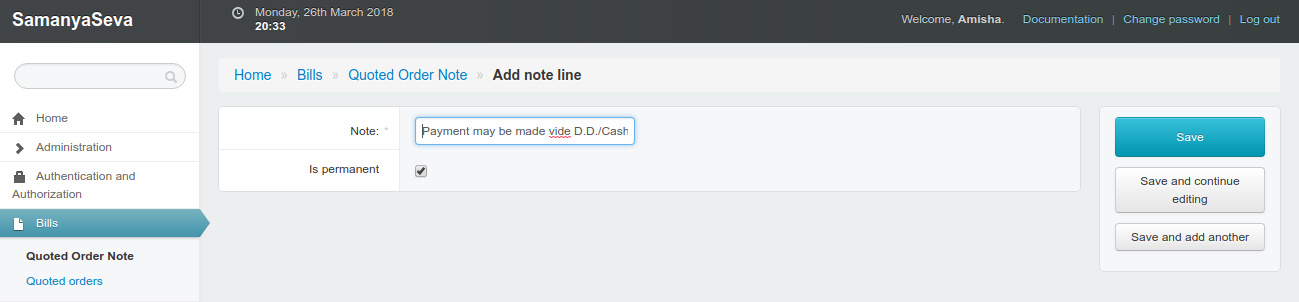
\includegraphics[scale=0.4]{input/images/bills_add.png}
\caption{ Bills}
\label{fig:UI1}
\end{figure}

\begin{figure}[h!]
\centering 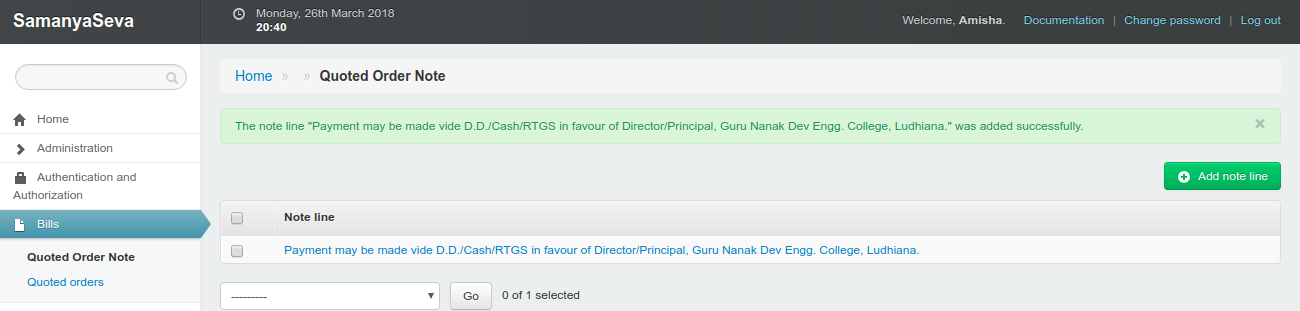
\includegraphics[scale=0.4]{input/images/bills_added.png}
\caption{ Billing Module}
\label{fig:UI1}
\end{figure}

\subsection{Suspense}
One can add the record department wise and can have a look over that.

\begin{figure}[h!]
\centering 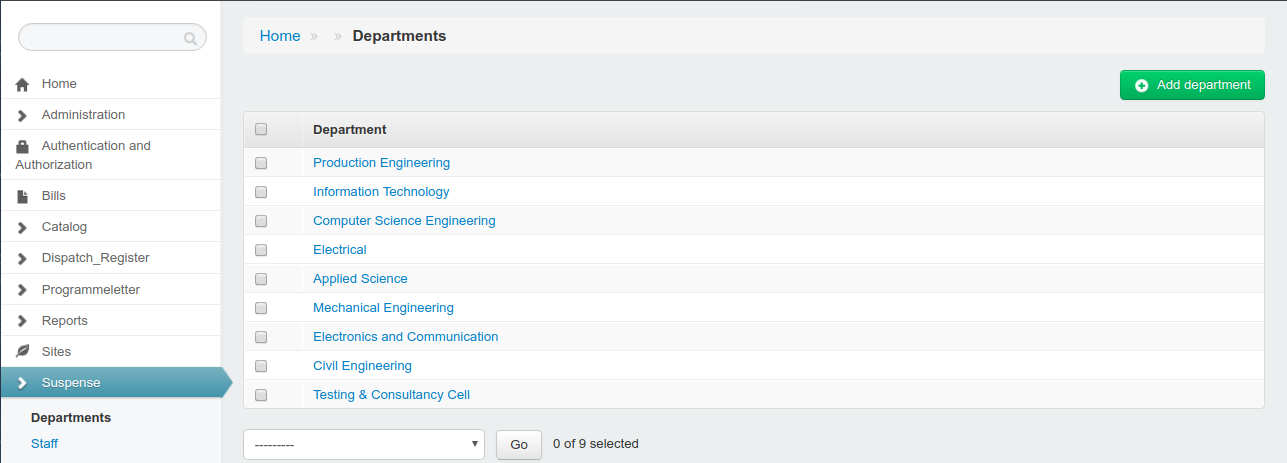
\includegraphics[scale=0.4]{input/images/suspense_dept.png}
\caption{ Departments}
\label{fig:UI1}
\end{figure}

\begin{figure}[h!]
\centering 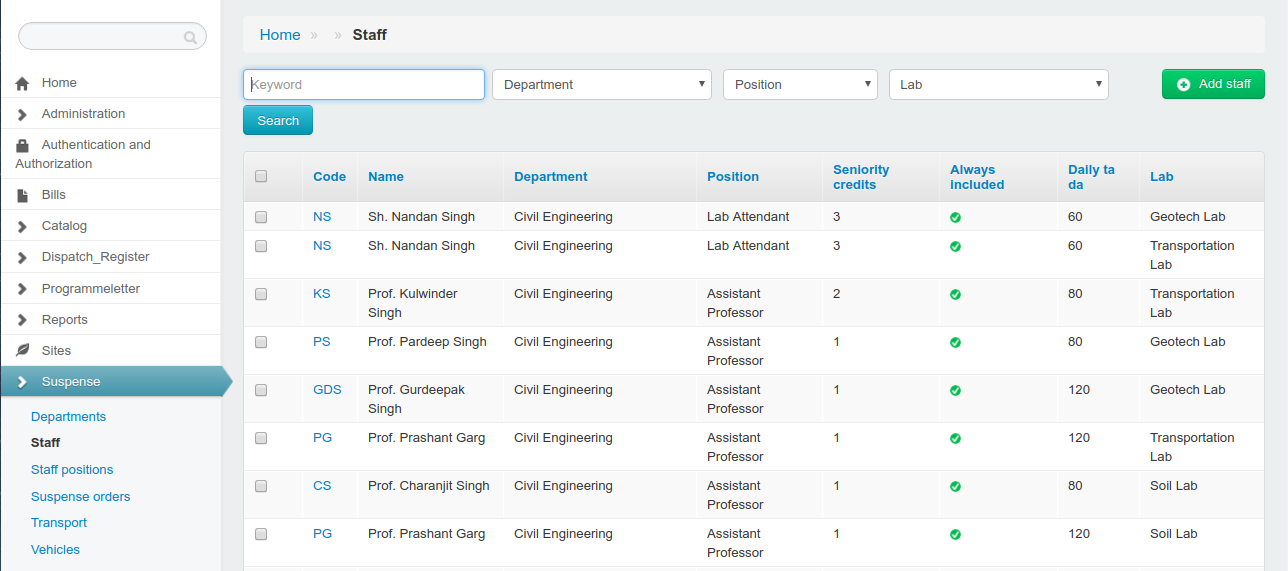
\includegraphics[scale=0.4]{input/images/suspense_staff.png}
\caption{ Suspense Module}
\label{fig:UI1}
\end{figure}

\subsection{Reports}
Here, Give a unique name to your report and have a excel type ready to use report in return.\\
There are many fields provided for user's ease such as:
\begin{itemize}
	\item First name
	\item Last name
	\item Title
	\item Street Address
	\item District
	\item Province
\end{itemize}
\begin{figure}[h!]
\centering 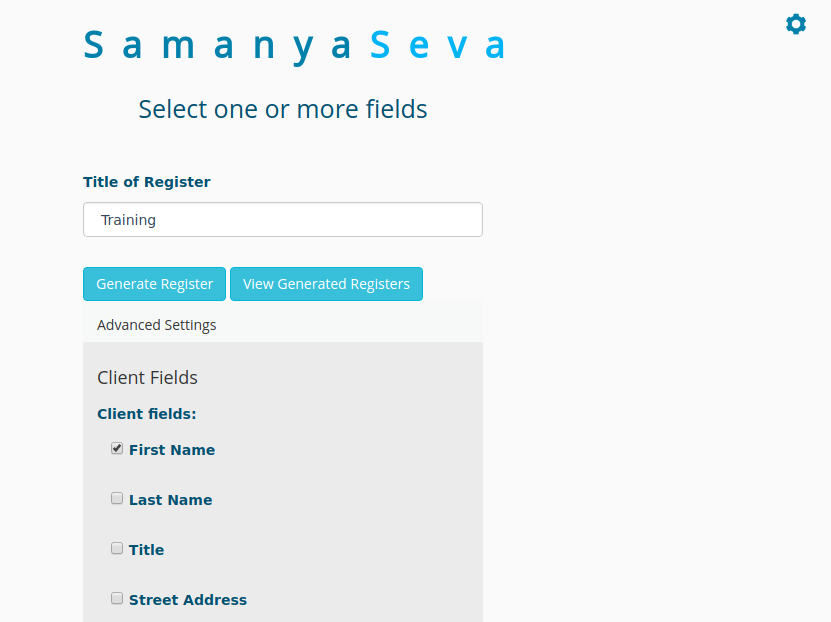
\includegraphics[scale=0.4]{input/images/gen1.png}
\caption{Generate Report}
\label{fig:UI1}
\end{figure}

\begin{figure}[h!]
\centering 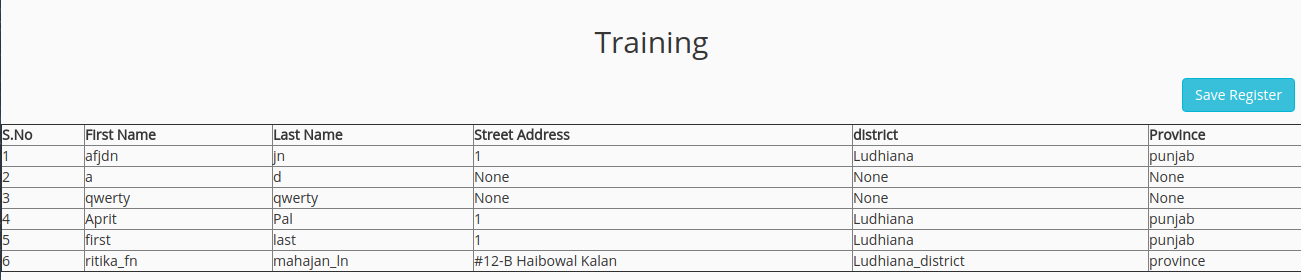
\includegraphics[scale=0.3]{input/images/gen2.png}
\caption{Generated Report}
\label{fig:UI1}
\end{figure}
\newpage
\subsection{Generate Registers}
\begin{figure}[h!]
\centering 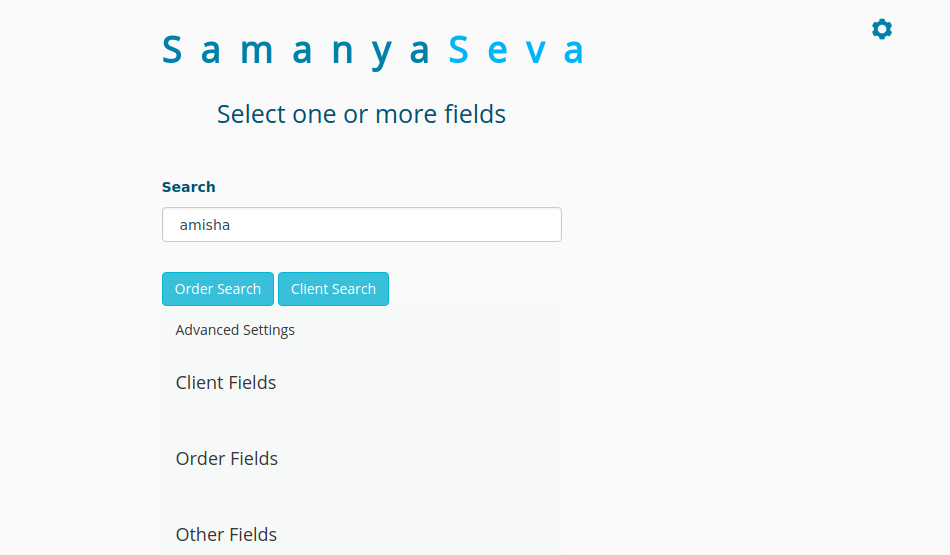
\includegraphics[scale=0.4]{input/images/search_client.png}
\caption{ Search Client}
\label{fig:UI1}
\end{figure}

\begin{figure}[h!]
\centering 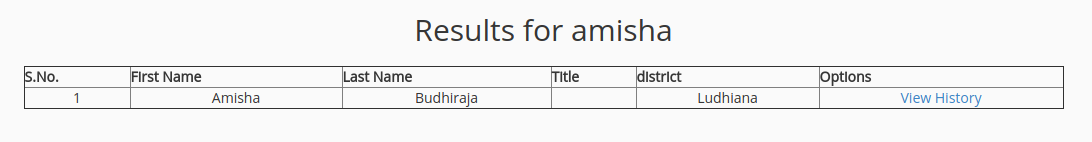
\includegraphics[scale=0.4]{input/images/search_result_1.png}
\caption{ Register}
\label{fig:UI1}
\end{figure}
\newpage

\section{Snapshots of Database Tables with brief description}

This depicts almost all the tables been created for this project. There are different tables made for different modules.\\
A proper naming structure with standards have been used for easy understanding about the working of this system. There are different tables shown below like for Bills module, User Module etc.
\begin{figure}[h!]
\centering 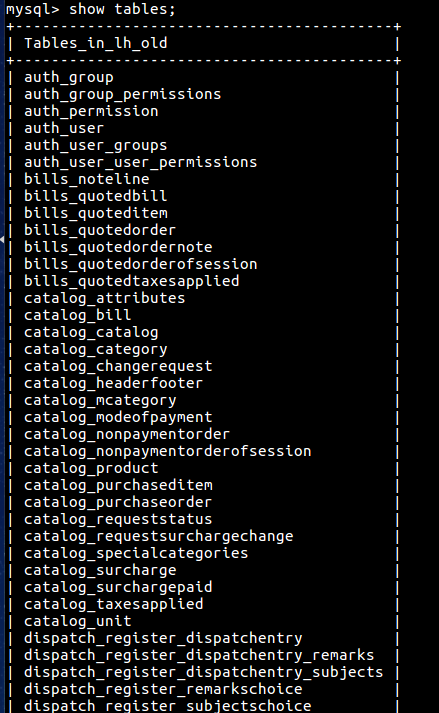
\includegraphics[scale=0.4]{input/images/t1.png}
\caption{ List of Tables}
\label{fig:UI1}
\end{figure}

Below is an important module which distinguishes our project from many i.e Catalog.\\
It's basically a menu driven module.

\begin{figure}[h!]
\centering 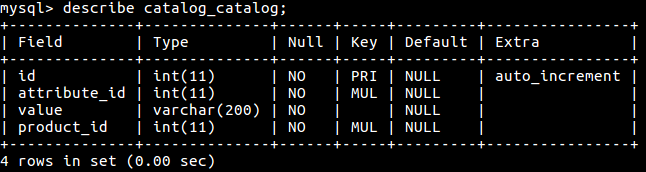
\includegraphics[scale=0.4]{input/images/t2.png}
\caption{ Catalog}
\label{fig:UI1}
\end{figure}

\begin{figure}[h!]
\centering 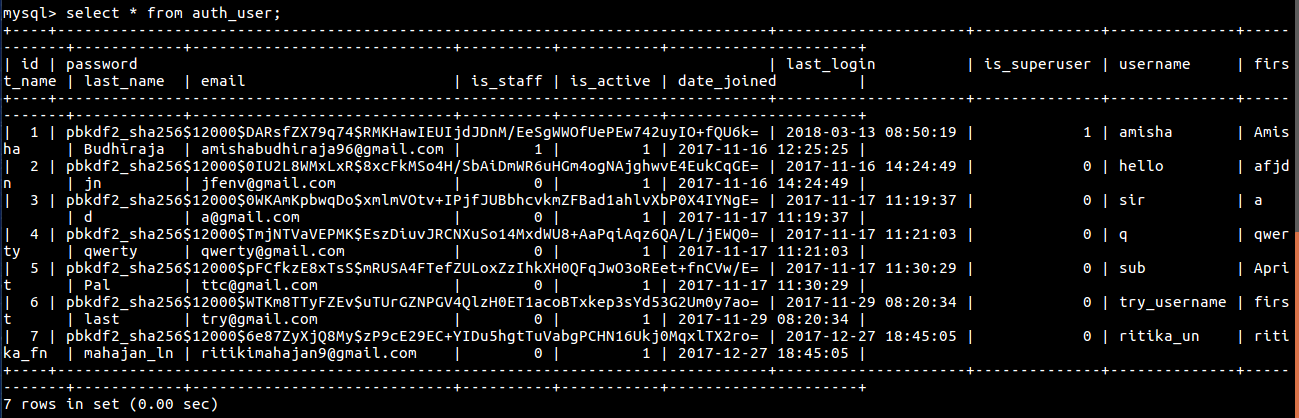
\includegraphics[scale=0.4]{input/images/t3.png}
\caption{ Auth User}
\label{fig:UI1}
\end{figure}
It's table of exisiting users with fields like First and last name, username etc.
\newpage

\section{BackEnd Representation}
\begin{figure}[h!]
\centering 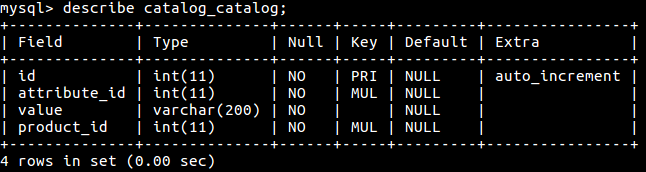
\includegraphics[scale=0.4]{input/images/t2.png}
\caption{ Catalog}
\label{fig:UI1}
\end{figure}

Known for it's performance, reliability and ease: MySQL is the world's most popular open source database. With its proven performance, reliability, and ease-of-use, MySQL has become the leading database choice for web-based applications, used by high profile web properties including Facebook, Twitter, YouTube, and all five of the top five websites.
A no. of tables has been made for each module separately and the database used for the same is MySQL.

\section{}